\documentclass[hidelinks,12pt]{article}
\usepackage[left=0.25cm,top=1cm,right=0.25cm,bottom=1cm]{geometry}
%\usepackage[landscape]{geometry}
\textwidth = 20cm
\hoffset = -1cm
\usepackage[utf8]{inputenc}
\usepackage[spanish,es-tabla, es-lcroman]{babel}
\usepackage[autostyle,spanish=mexican]{csquotes}
\usepackage[tbtags]{amsmath}
\usepackage{nccmath}
\usepackage{amsthm}
\usepackage{amssymb}
\usepackage{mathrsfs}
\usepackage{graphicx}
\usepackage{subfig}
\usepackage{caption}
%\usepackage{subcaption}
\usepackage{standalone}
\usepackage[outdir=./Imagenes/]{epstopdf}
\usepackage{siunitx}
\usepackage{physics}
\usepackage{color}
\usepackage{float}
\usepackage{hyperref}
\usepackage{multicol}
\usepackage{multirow}
%\usepackage{milista}
\usepackage{anyfontsize}
\usepackage{anysize}
%\usepackage{enumerate}
\usepackage[shortlabels]{enumitem}
\usepackage{capt-of}
\usepackage{bm}
\usepackage{mdframed}
\usepackage{relsize}
\usepackage{placeins}
\usepackage{empheq}
\usepackage{cancel}
\usepackage{pdfpages}
\usepackage{wrapfig}
\usepackage[flushleft]{threeparttable}
\usepackage{makecell}
\usepackage{fancyhdr}
\usepackage{tikz}
\usepackage{bigints}
\usepackage{menukeys}
\usepackage{tcolorbox}
\tcbuselibrary{breakable}
\usepackage{scalerel}
\usepackage{pgfplots}
\usepackage{pdflscape}
\pgfplotsset{compat=1.16}
\spanishdecimal{.}
\renewcommand{\baselinestretch}{1.5} 
\renewcommand\labelenumii{\theenumi.{\arabic{enumii}})}

\newcommand{\python}{\texttt{python}}
\newcommand{\textoazul}[1]{\textcolor{blue}{#1}}
\newcommand{\azulfuerte}[1]{\textcolor{blue}{\textbf{#1}}}
\newcommand{\funcionazul}[1]{\textcolor{blue}{\textbf{\texttt{#1}}}}

\newcommand{\pderivada}[1]{\ensuremath{{#1}^{\prime}}}
\newcommand{\sderivada}[1]{\ensuremath{{#1}^{\prime \prime}}}
\newcommand{\tderivada}[1]{\ensuremath{{#1}^{\prime \prime \prime}}}
\newcommand{\nderivada}[2]{\ensuremath{{#1}^{(#2)}}}


\newtheorem{defi}{{\it Definición}}[section]
\newtheorem{teo}{{\it Teorema}}[section]
\newtheorem{ejemplo}{{\it Ejemplo}}[section]
\newtheorem{propiedad}{{\it Propiedad}}[section]
\newtheorem{lema}{{\it Lema}}[section]
\newtheorem{cor}{Corolario}
\newtheorem{ejer}{Ejercicio}[section]

\newlist{milista}{enumerate}{2}
\setlist[milista,1]{label=\arabic*)}
\setlist[milista,2]{label=\arabic{milistai}.\arabic*)}
\newlength{\depthofsumsign}
\setlength{\depthofsumsign}{\depthof{$\sum$}}
\newcommand{\nsum}[1][1.4]{% only for \displaystyle
    \mathop{%
        \raisebox
            {-#1\depthofsumsign+1\depthofsumsign}
            {\scalebox
                {#1}
                {$\displaystyle\sum$}%
            }
    }
}
\def\scaleint#1{\vcenter{\hbox{\scaleto[3ex]{\displaystyle\int}{#1}}}}
\def\scaleoint#1{\vcenter{\hbox{\scaleto[3ex]{\displaystyle\oint}{#1}}}}
\def\scaleiiint#1{\vcenter{\hbox{\scaleto[3ex]{\displaystyle\iiint}{#1}}}}
\def\bs{\mkern-12mu}

\newcommand{\Cancel}[2][black]{{\color{#1}\cancel{\color{black}#2}}}


\usetikzlibrary{patterns}

\title{\vspace{-2cm} Examen Parcial 1 - 2024-1 \\ {\large Curso Física Computacional} \vspace{-3ex}}
\author{M. en C. Gustavo Contreras Mayén. \texttt{gux7avo@ciencias.unam.mx}}
\date{}

\begin{document}

\fontsize{14}{14}\selectfont
\vspace{-4cm}
\maketitle

Instrucciones: resuelve cada ejercicio apoyándote con un código en python, deberás de identificar cada archivo de la forma: \texttt{ejercicio1.py}, \texttt{ejercicio2.py}, etc. para que envíes un solo archivo compactado con las soluciones. 
\begin{enumerate}
\item Las siguientes expresiones definen a la constante de Euler:
\begin{align}
\gamma &= \lim_{n \rightarrow \infty} \left[ \nsum_{k=1}^{n} \dfrac{1}{k} - \ln (n) \right] \\
\gamma &= \lim_{k \rightarrow \infty} \left[ \nsum_{k=1}^{m} \dfrac{1}{k} - \ln \left( m + \dfrac{1}{2} \right) \right]
\end{align}
Escribe un programa que calcule el valor de $\gamma = 0.57721$, ¿cuál de las dos expresiones converge más rápido al valor?
\item El valor de $\pi$ se puede calcular aproximando el área de un círculo unitario como el límite de una sucesión $p_{1}, p_{2}, \ldots$ descrita a continuación:
\par
Se divide un círculo unitario en $2^{n}$ sectores (en el ejemplo, $n=3$). Se aproxima el área del sector por el área del triángulo isóceles. El ángulo $\theta_{n}$ es $2 \pi / 2^{n}$. El área del triángulo es $1/2 \sin \theta_{n}$.
\\
\begin{figure}[H]
\centering
\includestandalone{Figuras/circulo_pi}
\caption{División en $n$ sectores.}
\end{figure}
La enésima aproximación a $\pi$ es: $p_{n}= 2^{n-1} \sin \theta_{n}$.
\begin{enumerate}
\item Demuestra que
\[\sin \theta_{n} = \dfrac{\sin \theta_{n - 1}}{\left( 2 \left[ 1 + (1 - \sin^{2}\theta_{n - 1})^{\frac{1}{2}} \right] \right)^{\frac{1}{2}}} \]
\item Usa esta relación de recurrencia para generar las sucesiones $\sin \theta_{n}$ y $p_{n}$ en el rango $3 \leq n \leq 20$ iniciando con $\sin \theta_{2} = 1$. Compara tus resultados con el valor de $4.0 \: \arctan(1.0)$
\end{enumerate}
%\item Encontrar la raíz de $y (x)$ a partir de los siguientes datos:
%\begin{table}[H] 
%\centering 
%\begin{tabular}{c | c | c | c | c | c | c | c |}
%$x$ & $0$ & $0.5$ & $1$ & $1.5$ & $2$ & $2.5$ & $3$ \\ \hline
%$y$ & $1.8421$ & $2.4694$ & $2.4921$ & $1.9047$ & $0.8509$ & $-0.4112$ & $-1.5727$ 
%\end{tabular}
%\end{table}
%Usando la interpolación de Lagrange sobre a) tres puntos, y b) sobre cuatro puntos vecinos más cercanos.
\item La siguiente tabla muesta como la densidad relativa $\rho$ del aire varía con la altitud $h$. Calcula la densidad relativa del aire en $10.5$ km.
\begin{table}[H]
\centering 
\begin{tabular}{c | c | c | c | c | c | c | c |}
$h (km)$ & $0$ & $1.525$ & $3.050$ & $4.575$ & $6.10$ & $7.625$ & $9.150$ \\ \hline
$\rho$ & $1$ & $0.8617$ & $0.7385$ & $0.6292$ & $0.5328$ & $0.4481$ & $0.3741$ 
\end{tabular}
\end{table}
\item Determina las raíces de las siguientes ecuaciones mediante el método de la falsa posición modificada:
\begin{enumerate}
\renewcommand{\arraystretch}{1.5}
\item $f(x) = \exp(x) - 5 \, x^{2} = 0$
\item $h(x) = x^{3} + 2 \, x - 1 = 0$
\end{enumerate}
\item Identifica el intervalo para las raíces de las siguientes ecuaciones y calcula después las raíces mediante el método de la secante, con una tolerancia de $0.001$:
\begin{enumerate}
\item $0.1 \, x^{3} - 5 \, x^{2} - x + 4 + \exp(-x) = 0$
\item $\ln(x) -0.2 \, x^{2} + 1 = 0$
\end{enumerate}
\item Considera la siguiente imagen:
\begin{figure}[H]
	\centering
	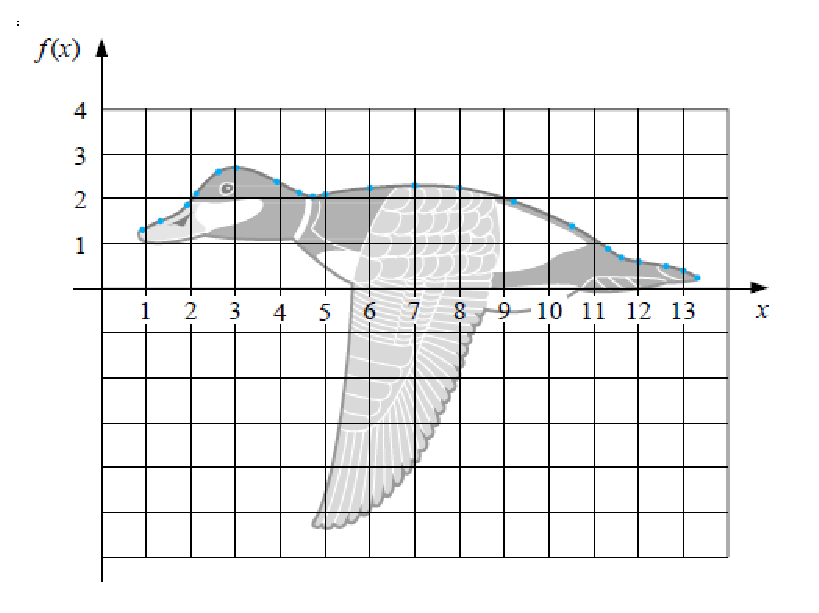
\includegraphics[scale=0.7]{Imagenes/ContornoPato.eps}  
\end{figure}
Hay que encontrar una función que represente el contorno del pato en el primer cuadrante, para ello debes:
\begin{enumerate}
\item Definir un conjunto de puntos (entre $15$ - $20$ puntos)
\item Usar la técnica de interpolación de Lagrange para revisar si la función de interpolación, representa debidamente el contorno.
\item Usar la técnica de interpolación con splines.
\end{enumerate}
\item Usando una aproximación por diferencias finitas de orden $O(h^{2})$, calcula $\pderivada{f} (2.36)$ y $\sderivada{f} (2.36)$, a partir de los datos:
\begin{table}[H]
\centering
\begin{tabular}{c | c | c | c | c}
$x$ & $2.36$ & $2.37$ & $2.38$ & $2.39$ \\ \hline 
$f (x)$ & $0.85866$ & $0.86289$ & $0.86710$ & $0.87129$
\end{tabular}
\end{table}

\item La palanca $AB$ de longitud $R = \SI{90}{\milli\meter}$ está girando con velocidad angular constante $\dv*{\theta}{t} = 5000$ rev/min.
\begin{figure}[H]
\centering
\begin{tikzpicture}[font=\small, scale=1.4, fill=]
\draw (-0.4,-0.3) [pattern= north east lines] rectangle (0.6,0);
\draw (-0.1,0) -- node [above left]{A} (-0.1,0.3)arc (180:0:0.2cm) -- (0.3,0);
\draw (0.1,0.3) circle (0.05);
\draw [dashed] (0.1,0.3) -- node [midway, below] {x} (3.3,0.3);
\draw (3.3,0.3) circle (0.05);
\draw (1.15,1.45) circle (0.05);
\draw (0.1,0.49) -- node [midway, above] {R}(1,1.42);
\draw (0.27,0.4) -- (1.18,1.32);
\draw (1,1.42) -- (3.35,0.15) [rotate=-120] arc  (0:180:0.1cm);
\draw (3.47,0.31) -- node[midway, above, sloped]{2.5R}(1.1,1.6) [rotate=60] arc (0:180:0.1cm);
\draw (1,1.9) node {B};
\draw (2.8,-0.2) [pattern= north east lines] rectangle (4.5,-0.1);
\draw (3.05,0.65) [pattern= north east lines] rectangle (4.5,0.55);
\draw [thick] (3.1,0.3) -- (3.1,-0.07) -- (4.3,-0.07) -- node [midway, right]{C}(4.3,0.55) -- (3.1,0.55);
\draw [thick] (3.8,-0.07) -- (3.8,0.55);
\draw [thick] (3.9,-0.07) -- (3.9,0.55);
\draw [thick] (4,-0.07) -- (4,0.55);
\draw (0.5,0.3) arc (0:70:0.2cm);
\draw (0.7,0.5) node {$\theta$};
\end{tikzpicture}
\end{figure}
La posición del pistón $C$ como se muestra, varía con el ángulo $\theta$:
\begin{align*}
x = R \, \left( \cos \theta + \sqrt{2.5^{2} - \sin^{2} \theta} \right)
\end{align*}
Calcula mediante diferenciación numérica la aceleración del pistón en:  $\theta = \ang{0}, \ang{5}, \ang{10}, \ldots, \ang{180}$.
\item Las estaciones de radar \textit{A} y \textit{B} están separadas por una distancia $a = \SI{500}{\meter}$; rastrean el avión \textit{C} registrando los ángulos $\alpha$ y $\beta$ en intervalos de un segundo. Si hay tres lecturas sucesivas:
\begin{table}[H]
\centering
\begin{tabular}{c l l l }
$t(s)$ & $9$ & $10$ & $11$ \\ \hline
$\alpha$ & $\ang{54.80}$ & $\ang{54.06}$ & $\ang{53.34}$ \\ \hline
$\beta$ & $\ang{65.59}$ & $\ang{64.59}$ & $\ang{63.62}$
\end{tabular}
\end{table}
\begin{figure}[H]
	\centering
	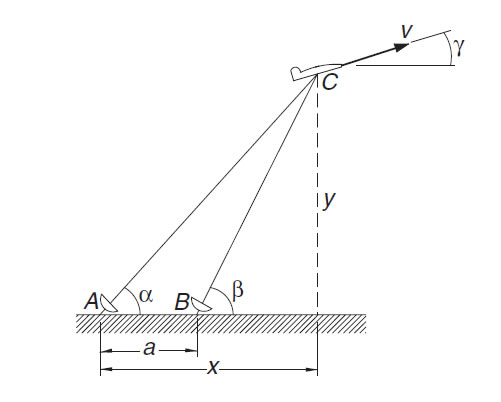
\includegraphics[scale=0.6]{Imagenes/ExamenFinal02_01.jpg} 
	\caption{Estaciones de radar y el avión.}
\end{figure}
Calcula la velocidad $v$ del avión y el ángulo de subida $\gamma$ en $t = 10$ segundos. Las coordenadas del avión las tomamos de
\[x = a \, \dfrac{\tan \beta}{\tan \beta - \tan \alpha} \hspace{1.5cm} y= a \, \dfrac{\tan \alpha \tan \beta}{\tan \beta - \tan \alpha}\]


\item La siguiente tabla indica la potencia $P$ propocionada por las ruedas de un carro como función de la velocidad $v$. Si la masa del carro es $m = 2000$ kg, calcula el tiempo $\Delta t$ necesario para que el carro acelere de $\SI{1}{\meter\per\second}$ m/s a $\SI{6}{\meter\per\second}$ m/s. Usa la regla del trapecio para integrar. Tip:
\begin{align*}
\Delta t = m \, \scaleint{6ex}_{\bs 1s}^{6s} \left( \dfrac{v}{P} \right) \dd{v}
\end{align*}
que se puede obtener de la segunda ley de Newton y por la definición de potencia, $P = F \, v$.
\begin{center}
\begin{tabular}{c | c | c | c | c | c | c | c | c}
$v$ (m/s) & 0 & 1.0 & 1.8 & 2.4 & 3.5 & 4.4 & 5.1 & 6.0 \\ \hline
$P$ (kW)  & 0 & 4.7 & 12.2 & 19.0 & 31.8 & 40.1 & 43.8 & 43.2 
\end{tabular}
\end{center}
\item El período de un péndulo de longitud $L$ es:
\begin{align*}
\tau = 4 \, \sqrt{\dfrac{L}{g}} \, h(\theta_{0})
\end{align*}
donde $g$ es la aceleración debida a la gravedad, $\theta_{0}$, representa la amplitud angular y 
\begin{align*}
h (\theta_{0}) =  \scaleint{6ex}_{\bs 0}^{\frac{\pi}{2}} \dfrac{\dd{\theta}}{\sqrt{1 - \sin^{2} \left( \frac{\theta_{0}}{2}\right) \sin^{2} \theta}}
\end{align*}
Calcula $h (\ang{15})$, $h (\ang{30})$ y $h (\ang{45})$; compara esos valores con $h (\ang{0}) = \dfrac{\pi}{2}$ (la aproximación usada para pequeñas amplitudes)
\end{enumerate}

\end{document}